% LREC 2022 KC Example; 
% LREC Is now using templates similar to the ACL ones. 
\documentclass[10pt, a4paper]{article}
\usepackage{lrec2022} % this is the new LREC2022 Style
\usepackage{multibib}
\newcites{languageresource}{Language Resources}
\usepackage{graphicx}
\usepackage{tabularx}
\usepackage{soul}
\usepackage{todonotes}
\usepackage{cjhebrew}
\usepackage{tipa}
% for eps graphics
%%% References and Labels
%%% Reference labels without a punctuation 
% courtesy of Marc Schulder , uni Hamburg ****************
\usepackage{titlesec}
%\titleformat{\section}{\normalfont\large\bf\center}{\thesection.}{1em}{}
\titleformat{\section}{\normalfont\large\bfseries\center}{\thesection.}{1em}{}
\titleformat{\subsection}{\normalfont\SmallTitleFont\bfseries\raggedright}{\thesubsection.}{1em}{}
\titleformat{\subsubsection}{\normalfont\normalsize\bfseries\raggedright}{\thesubsubsection.}{1em}{}
\renewcommand\thesection{\arabic{section}}
\renewcommand\thesubsection{\thesection.\arabic{subsection}}
\renewcommand\thesubsubsection{\thesubsection.\arabic{subsubsection}}
%  ed 

\usepackage{epstopdf}
\usepackage[utf8]{inputenc}

\usepackage{hyperref}
\usepackage{xstring}

\usepackage{color}

\newcommand{\secref}[1]{\StrSubstitute{\getrefnumber{#1}}{.}{ }}

\title{\vspace*{.5\baselineskip} \textbf{Lexical Semantic Change Detection in Resource-Light, Morphologically Rich Languages: A Case Study in Emergent Modern Hebrew}}
\name{Raz Besaleli, Zachary Schultz, Anna Feldman, Jing Peng}

\address{Montclair State University \\
        1 Normal Ave \\
        Montclair, NJ 07043, USA \\
         % Address1, Address2, Address3 \\
         % author1@xxx.yy, author2@zzz.edu, author3@hhh.com\\
         \{besalelir1,schultzz1,feldmana,pengj\}@montclair.edu\\}



\abstract{
In the past few years, lexical semantic change detection (LSCD) using contextualized word embeddings has been a topic that has gained a lot of interest in the NLP community. In this paper, we discuss the challenges of applying LSCD with contextualized word embeddings to Modern Hebrew, whose complex history, resource-light nature, rich morphology, and ambiguous morphology impose several significant experimental limitations.
 \\ \newline \Keywords{Emergent Modern Hebrew, Lexical Semantic Change Detection, NLP} }

\begin{document}

\maketitleabstract

\section{Introduction}

\subsection{On Emergent Modern Hebrew}
Modern Hebrew (MH) is a morphologically rich, resource-light language belonging to the Semitic branch of the Afro-Asiatic family. Its grammar is fusional and synthetic, with a nonconcatenative, autosegmental\footnote{explain autosegmental morphology here} morphology \cite{nonlinearmorphology}, and a complex verbal template system that both often lead to significant morphological ambiguity. MH's orthography also contributes to this ambiguity, as it is an (impure) abjad that does not notate all vowels.
These traits make MH a particularly challenging language to work with in NLP. They, along with "language-agnostic" tools' general incompatibility with MH, have contributed to a significant deficiency of NLP resources for the language \cite{tsarfaty2019whats}.
Emergent Modern Hebrew, a particular chronolect of Modern Hebrew, is a historical period in which Hebrew was exposed to a significant amount of language contact due to significant political events such as war and mass immigration. It can be defined as beginning around 1881, marking the birth of the first native MH speaker, to around 1949, marking the establishment of the State of Israel. Although the nascence of Modern Hebrew in the early-mid 19th century has been widely studied, Emergent Hebrew has suffered a lack of research, mostly due to a lack of resources \cite{Rubinstein2019}.

\subsection{The Jerusalem Corpus of Emergent Modern Hebrew}
The Jerusalem Corpus of Emergent Modern Hebrew, is an annotated, multigenre corpus of Modern Hebrew texts written between the early 1720s to the late 1970s. It is composed of several subcorpora \cite{Rubinstein2019}:
\begin{itemize}
    \item \textbf{Street Ads:} A corpus of ephemera (street ads, posters, etc.) from 1862-1941.
    \item \textbf{Municipal Posters:} A corpus of ephemera from 1920-1960.
    \item \textbf{Dated BYP:} A corpus of literature, poetry, opinions, and journalism, taken from the Ben-Yehuda Project, from 1830-1970.
\end{itemize}

In this paper, we focus on an analysis of the Dated BYP subcorpus, in the time range 1881-1949, and omit the other subcorpora.
\subsection{Code}
The following repositories contain the code we used for this experiment:
\begin{itemize}
    \item The proprietary data frame for word usage matrices and corpus, code for distance measures, and code for extracting BERT embeddings can be found at \href{https://github.com/rbesaleli/dcwetk}{https://github.com/rbesaleli/dcwetk}.
    \item The code for the experiments can be found at \href{https://github.com/rbesaleli/LSCD-EmergentModernHebrew}{https://github.com/rbesaleli/LSCD-EmergentModernHebrew}.
\end{itemize}
\section{Related Work}
Applying unsupervised machine learning methods to contextualized word embeddings has proven to be an effective technique for diachronic LSCD, and has been shown to positively correlate with human judgments regarding diachronic semantic shift \cite{Giulianelli2020,Kutuzov2020}, especially when the contextualized word embeddings are extracted from ELMo \cite{Kutuzov2020}. The specific methods used are diverse, ranging from tracking the movement of word embedding clouds through semantic space, to measuring change in word usage distributions over time via word-sense induction using clustering.

There are several clustering methods that have been used for the latter method mentioned above. Clustering methods that require a user-defined number of clusters, such as K-Means Clustering \cite{Giulianelli2020} or Agglomerative Clustering \cite{Laicher2021}, may be paired with the Silhouette Method to find the optimal number of clusters. Alternatively, a clustering method that predetermines the number of clusters may be used, such as Affinity Propagation \cite{Martinc2020,Kutuzov2020}. This is discussed further in \ref{clustering}.

That said, the performance of type-based embeddings has been shown to exceed the performance of token-based embeddings in LSCD, although the performance of the latter can be significantly improved by reducing word-form bias through methods such as lemmatization \cite{Laicher2021}, and in certain cases, fine-tuning the model \cite{Martinc2020}. 

An alternative to LSCD that utilizes grammatical profiling instead of contextualized word embeddings has been shown to be just as effective, if not more \cite{grammaticalprofiling}, with the added benefit that semantic change that is detected is significantly more traceable than its counterpart that uses contextualized word embeddings. That said, its performance is contingent on understanding which grammatical features are correlated to semantic change. Which features are significant varies from language to language, and thus requires resources such as an existing corpus that is annotated with semantic information.

It should also be noted that many of these related works are concerned with languages such as German, Swedish, and English, that had access to resources such as SemEval, and therefore had the ability to correlate their findings with human-annotated gold standards. Modern Hebrew does not have this luxury, which puts a significant limitation on what we are able to observe.
\section{Experimental Design}

\subsection{Preprocessing the JEMH}

\subsubsection{Lemmatization}
After tokenization, the corpus is lemmatized in order to relieve any bias created by Hebrew's morphological richness \cite{Laicher2021}. To do this, we utilize Yet Another Parser (YAP), a morphological analyzer for Modern Hebrew, written in Go \cite{yap}. Word forms, lemmas, POS tags, and any relevant morphological features are collected from YAP's morphological disambiguator. \todo{say 1-2 sentences  the lemmatizer works. I think it first provides lexicon-based morphological analysis followed by a disambiguation step involving morphosyntactic parsing?} 

\subsubsection{Generating Contextualized Word Embeddings}
To generate contextualized word embeddings, we fed the lemmatized corpus through AlephBERT, a large distribution of BERT, pre-trained on a variety of corpora, including Modern Hebrew Twitter, Wikipedia, and OSCAR \cite{alephBERT}. The raw contextualized word embeddings themselves were generated from its hidden states. We choose to omit any fine-tuning of the BERT model, due to its mixed results.

\subsection{Word Usage Set}
Given a token $w$ and a time period $t$, we define word usage set\footnote{Word usage sets may also be known as 'word usage matrices' in other relevant literature \cite{Kutuzov2020,Giulianelli2020}. A similar concept, known as Word Usage Graphs, are used by authors such as \newcite{Laicher2021}.} $\textbf{U}^{t}_w$, where a word usage set is a set containing the contextualized word embeddings of all instances of a given token $w$ in time period $t$, and its size (i.e., number of embeddings) $N^t_w$.

\subsubsection{Prototype}
The prototype of a word usage set, which may be interpreted as a "context-averaged embedding" of a given token $w$, is calculated as follows:

$$\textbf{p}^t_w = \frac{\sum_{x_i \in \textbf{U}^t_w} x_i}{N^t_w}$$

\subsection{Measuring Distance}
\label{distance}
% need section on word usage matrix representation!!!
To measure diachronic lexical semantic change of a token, we use 4 different methods, per \newcite{Kutuzov2020,Giulianelli2020}. Given all embedded instances of a token $w$ in two time periods $t, t'$, we define word usage sets $\textbf{U}^{t}_w, \textbf{U}^{t'}_w$.

\subsubsection{Inverse Cosine Over Word Prototypes}
Inverse Cosine Over Word Prototypes (PRT) measures the inverted cosine similarity $d$ between the prototypes ("averages") of two given word sets $\textbf{U}^{t}_w, \textbf{U}^{t'}_w$:
$$\textsc{PRT}(\textbf{U}^{t}_w, \textbf{U}^{t'}_w) = d(p^{t}_w, p^{t'}_w)^{-1}$$
% $$PRT(\textbf{u}^{t}_w, \textbf{u}^{t'}_w) = d(\frac{\sum_{x_i \in \textbf{u}^{t}_w} x_i}{N^{t}_{w}}, \frac{\sum_{x_i \in \textbf{u}^{t'}_w} x_i}{N^{t'}_{w}})^{-1}$$
% Because a prototype is a relatively shallow representation of a word usage matrix, PRT only gives an idea of the absolute diachronic movement of a word usage matrix in space, and does not explicitly embed how the structure of the word usage matrix changes over time. 
This may be interpreted as the cosine distance between a given token's "context-averaged embeddings" in two different time periods.

\subsubsection{Average Pairwise Cosine Distance Between Token Embeddings}
Average Pairwise Cosine Distance Between Token Embeddings (APD) sums all cosine distances between every possible pair of embeddings in each given word usage sets $\textbf{U}^{t}_w, \textbf{U}^{t'}_w$, which is then divided by the aggregate number of possible embedding pairs:
$$\textsc{APD}(\textbf{U}^{t}_w, \textbf{U}^{t'}_w) = \frac{1}{N^{t}_w \cdot N^{t'}_w} \sum_{x_i \in \textbf{U}^{t}_w, x_j \in \textbf{U}^{t'}_w} d(x_i, x_j)$$
Like PRT, since APD also utilizes a somewhat shallow understanding of each word usage set, it also does not embed any meaningful information of how the structure of the word usage set changes over time. Thus, it may be interpreted as the average distance each individual embedding moves over time.\\

Because APD has a significant computational load, with a worst-case time complexity of $O(n^2)$, we chose to run it on samples of each word usage sets in the event that $N^{t}_w \cdot N^{t'}_w > 256$. How large these samples were was calculated by the following formula for each pair of word usage matrices:
$$n(\textbf{U}^{t}_w, \textbf{U}^{t'}_w) = \frac{256}{N^{t}_w \cdot N^{t'}_w}$$
While not ideal, this gave us a reasonable cap on the number of possible computations that could occur that maintained the relative sizes of each word usage matrix. % reword this

\subsubsection{Jensen-Shannon Divergence}
\label{JSD}
Jensen-Shannon Divergence (JSD) measures how the distribution of word-senses for each word usage set $\textbf{U}^{t}_w, \textbf{U}^{t'}_w$ changes over time, where $H$ is the Boltzmann-Gibbs-Shannon Entropy \cite{jensenshannon}:
\small $$\textsc{JSD}(\textbf{U}^{t}_w, \textbf{U}^{t'}_w) = H(\frac{1}{2}(\textbf{U}^{t}_w + \textbf{U}^{t'}_w)) - \frac{1}{2}(H(\textbf{U}^{t}_w) - H(\textbf{U}^{t'}_w))$$
The word usage sets above must be clustered to obtain the distribution of word-senses mentioned above. How we obtained said clusterings is discussed in the \ref{clustering}.
\subsubsection{Difference between Token Embedding Diversities}
Difference between Token Embedding Diversity (DIV) measures the difference in the average distance of a given embedding in a word usage set to its prototype between two word usage sets $\textbf{U}^{t}_w, \textbf{U}^{t'}_w$:
% align with amsmath or reformat
$$\textsc{DIV}(\textbf{U}^{t}_w, \textbf{U}^{t'}_w) = $$ 
$$\Bigg | \frac{\sum_{x_i \in \textbf{U}^{t}_w} d(x_i, p^{t}_w)}{N^{t}_w} - \frac{\sum_{x_j \in \textbf{U}^{t'}_w} d(x_j, p^{t'}_w)}{N^{t'}_w} \Bigg |$$

\subsection{Clustering}
\label{clustering}
As mentioned in \ref{JSD}, in order to calculate the Jensen-Shannon Divergence between two given word usage sets, they must first be clustered in order to get their word usage distributions. There appears to be several schools of thought on how this should be done:
\begin{itemize}
    \item{Following \newcite{Martinc2020,Kutuzov2020}, the clusters could be obtained using Affinity Propagation. Although this has a significant time complexity, it does not require a predefined number of clusters.}
    \item{Following \newcite{Laicher2021}, the clusters could be obtained using Agglomerative Clustering, with the number of clusters found by the Silhouette Method\cite{silhouette}, an algorithm that determines the optimal number of clusters between a given range.}
    \item{Following \newcite{Giulianelli2020}, the clusters could be obtained by using K-Means Clustering, with the number of clusters found by the Silhouette Method. The clusters are then run through Expectation Maximization (EM) for 10 iterations to reduce distortion.}
\end{itemize}

After preprocessing a given word usage set pair $\textbf{U}^{t}_w, \textbf{U}^{t'}_w$ by subtracting the mean and normalizing them to unit variance, we chose to cluster the word usage sets together with Affinity Propagation (AP), following \cite{Martinc2020,Kutuzov2020}. Although the change in word usage is difficult to track due to the fact that AP naturally creates many clusters, it doesn't rely on an arbitrarily-set number of clusters which may not necessarily represent each sense in which a given word is used. To account for computational complexity, we randomly sampled each word usage matrix to a maximum size of 1,024 vectors (the maximum word usage set size to be clustered therefore has a maximum of 2,048 vectors).

\section{Observations}
\subsection{Distribution of Scores}
Upon looking at the distributions of lexical semantic change scores of all tokens in a given period of time, it is evident that the distribution APD and JSD scores of all tokens in a given period of time, describing the change in distribution of word-senses over a period of time, roughly fits a skewed normal distribution, shown by Figure \ref{1920_APD} and \ref{1920_JSD}, respectively. The skew of the distribution is much more prominent in the JSD scores, as shown in \ref{SkewKurtosis_JSDandAPD}. We hypothesize that this is due to the fact that Jensen-Shannon Divergence is not a metric, though its square root, Jensen-Shannon Distance (JSDist), is. As shown in \ref{1920_JSDist}, the distribution of Jensen-Shannon Distance values is significantly less skewed.


\begin{figure}[!h]
\begin{center}
%\fbox{\parbox{6cm}{
%This is a figure with a caption.}}
% old picture \includegraphics[scale=0.5]{lrec2020W-image1.eps} 
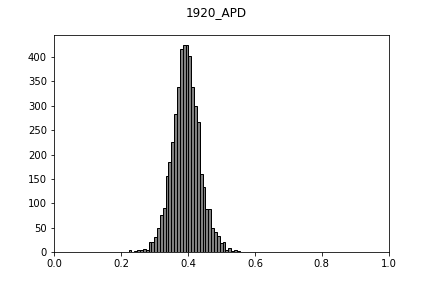
\includegraphics[scale=0.5]{code/distribution_imgs/1920_APD.png}
\caption{Distribution of APD scores (by token) from periods 1920-1925 to 1925-1930.}
\label{1920_APD}
\end{center}
\end{figure}

\begin{figure}[!h]
\begin{center}
%\fbox{\parbox{6cm}{
%This is a figure with a caption.}}
% old picture \includegraphics[scale=0.5]{lrec2020W-image1.eps} 
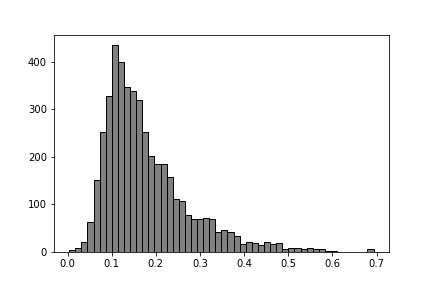
\includegraphics[scale=0.5]{code/distribution_imgs/1920_JSD.png}
\caption{Distribution of JSD scores (by token) from periods 1920-1925 to 1925-1930.}
\label{1920_JSD}
\end{center}
\end{figure}

\begin{figure}[!h]
\begin{center}
%\fbox{\parbox{6cm}{
%This is a figure with a caption.}}
% old picture \includegraphics[scale=0.5]{lrec2020W-image1.eps} 
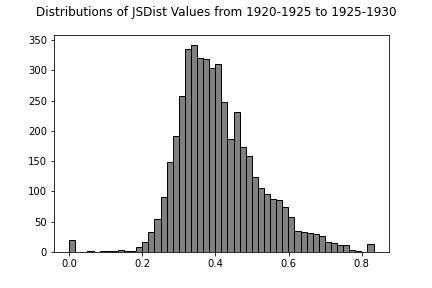
\includegraphics[scale=0.5]{code/distribution_imgs/1920_JSDist.png}
\caption{Distribution of JSDist scores (by token) from periods 1920-1925 to 1925-1930.}
\label{1920_JSDist}
\end{center}
\end{figure}

\begin{table}[!h]
\label{SkewKurtosis_JSDandAPD}
\begin{center}
\begin{tabularx}{\columnwidth}{|X|c|c|c|c|}

      \hline
       &\multicolumn{2}{c|}{JSD}&\multicolumn{2}{c|}{APD}\\
       \hline
      Year&Skew&Kurtosis&Skew&Kurtosis\\
      \hline
      1880&1.293&1.984&0.344&1.239\\
      \hline
      1885&1.339&2.456&0.243&0.728\\
      \hline
      1890&1.549&3.149&0.122&1.108\\
      \hline
      1895&1.691&3.868&-0.288&2.664\\
      \hline
      1900&1.751&4.011&-0.068&1.882\\
      \hline
      1905&1.749&4.092&-0.016&1.381\\
      \hline
      1910&1.568&3.472&0.023&1.609\\
      \hline
      1915&1.379&2.469&0.093&2.192\\
      \hline
      1920&1.559&3.090&0.016&1.070\\
      \hline
      1925&1.657&3.559&0.032&1.237\\
      \hline
      1930&1.330&2.419&0.006&1.820\\
      \hline
      1935&1.049&1.506&-0.012&1.421\\
      \hline
      1940&0.943&0.746&0.271&0.657\\
      \hline

\end{tabularx}
\caption{Skew and Kurtosis of JSD and APD value distributions over time}
 \end{center}
\end{table}

\subsection{Effects of Ambiguous Orthography on Clustering Efficacy}
As stated before, MH uses an abjad orthography that does not always notate vowels. This may lead to significant ambiguity, which is only augmented by MH's morphological richness. For example, the grapheme \</swnh> may have any of the following meanings:
\begin{itemize}
    \item /\textesh one/ repeat (verb, present participle, masculine singular)
    \item /\textesh ona/ repeat (verb, present participle, feminine singular)
    \item /\textesh one/ diverse, different (adjective, masculine singular)
    \item /\textesh one-/ diverse, different (construct state adjective, masculine singular)
    \item /\textesh ona/ diverse, different (adjective, feminine singular)
    \item /\textesh una/ it was changed (verb, perfect aspect, 3rd person masculine singular, variant spelling)
\end{itemize}

As shown in Figure \ref{embeddings_pos}\footnote{JJ, BN, VB, JJT, and BNT represent an adjective, participle, verb, construct adjective, and construct participle, respectively. Note that this is a PCA representation of the embeddings, and the relative distances of each embedding to another is approximate. The complete tagset used by YAP may be found on p. 7 of \newcite{treebank}.}, a sample of the embeddings for the token discussed above, these different meanings do not appear to have a clustered structure. 
To verify this, we randomly sampled 118 time-insensitive word usage sets (i.e., word usage matrices belonging to the epoch 1880-1950), annotated with parts of speech for each token instance. Each word usage matrix had instances with between 2-5 possible POS tags. We then clustered them via Affinity Propagation, the same clustering method we used for Jensen Shannon Divergence, which is discussed in Section \ref{JSD}. Defining a "homogeneous cluster" to be a cluster whose constituents all have the same part of speech, we then calculated the percentage of homogeneous clusters per $n$ number of parts of speech (again, $2 \leq n \leq 5$). Just 9\% of the clusters were homogeneous. Interestingly enough, however, there is a weakly positive correlation between the percentage of homogeneous clusters and number of parts of speech in a given cluster, with a Spearman Rank Correlation coefficient of 0.17.

\begin{figure}[!h]
\begin{center}
%\fbox{\parbox{6cm}{
%This is a figure with a caption.}}
% old picture \includegraphics[scale=0.5]{lrec2020W-image1.eps} 
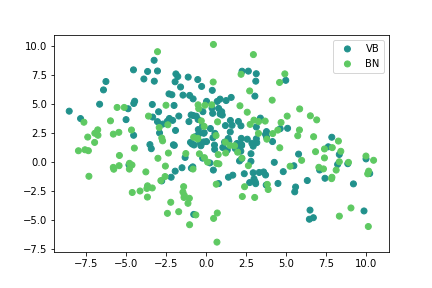
\includegraphics[scale=0.5]{code/embeddings_by_pos/שונה_1920.png}
\caption{PCA representation of contextualized word embeddings of the token \</swnh> in years 1920-1925}
\label{embeddings_pos}
\end{center}
\end{figure}

% \subsection{Some Examples}\todo{No transition from the previous section}
% Politically charged words, such as ethnic groups, governing bodies, and wars had particular interesting results. 
% \subsubsection{Example 1: Le'umi (trans. 'national')}
% The word "Le'umi" has several significantly different word-senses (not an exhaustive list): \todo{Since you lemmatized your data, I wonder what forms were merged into one. I'll include some links in an email  } 
% \begin{itemize}
%     \item Le'umi: National
%     \item Bank Le'umi: Name of a historical bank in Israel
%     \item Bituach Le'umi: Israeli health insurance system
% \end{itemize}

% This polysemy is further deepened by MH's morphological richness, whose explicit expressions were discarded during lemmatization. There is a certain ambiguity that also exists on another axis due to MH's orthographic ambiguity.

% As shown in Figure \ref{leumi}, the PRT and APD values of the word "le'umi" do not change much over time. While the explanation for the PRT feels rather obvious, considering the lack of movement shown in figures \ref{Leumi1} through \ref{Leumi5}, why the APD values over time remain stagnant is unclear. That said, the JSD measure was significantly more sensitive; it is easy to track the change in clusters over time. Overall, the word-senses of each time period do appear to be relatively stable.

% \subsubsection{Example 2: Aravi (trans. 'Arab')}
% Unlike the word "Le'umi", the word "Aravi" presents a more volatile semantic history, which is most obvious in the DIV and JSD measures, shown in Figure \ref{aravi}. Looking at the figures in the Appendix, it seems that this is caused by the word slowly forming distinct word-senses over time, peaking around 1935. Around that time was the Arab Revolt of 1936-1939, which may have contributed to the significant semantic drift.



% \begin{figure*}[ht]
% \begin{center}
% 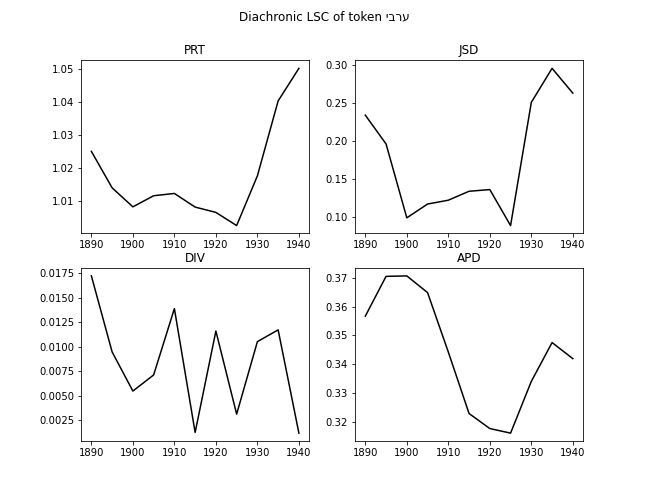
\includegraphics[scale=0.7]{code/distance_imgs/ערבי.png}
% \caption{Diachronic lexical semantic change of the word "Aravi".}
% \end{center}
% \label{aravi}
% \end{figure*}

% \begin{figure*}[ht]
% \begin{center}
% 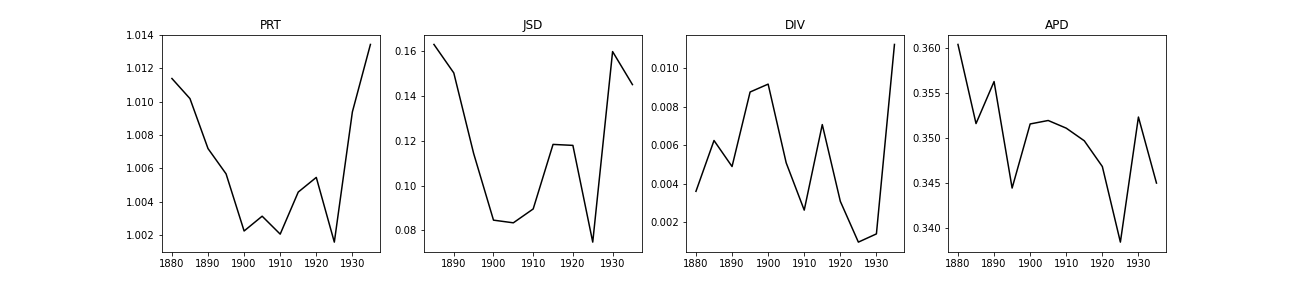
\includegraphics[scale=0.7]{code/distance_imgs/לאומי.png}
% \caption{Diachronic lexical semantic change of the word "Le'umi".}
% \end{center}
% \label{leumi}
% \end{figure*}

\section{Conclusion}
\subsection{Future Work}
While this experiment was interesting, again, it is not guaranteed that semantic change detected via contextualized word embeddings can be easily understood a priori without extensive manual work. Our findings could be juxtaposed with tracking semantic change via grammatical profiling, per \cite{grammaticalprofiling}. Particularly, there is some work on the semantic values of Hebrew verbal templates, known as \textit{binyanim}, that that they are worth investigating with computational methods. % cite this

%\section{Citing References in the Text}

%\subsection{Language Resource References}

%\subsubsection{When Citing Language Resources}
%As you may know, LREC introduced a separate section on Language Resources citation to enhance the value of such assets. When citing language resources, we recommend to proceed in the same way as for bibliographical references. Please make sure to compile your Language Resources stored as a .bib file \textbf{separately} (BibTex under pdfLaTeX). This produces the required .aux et .bbl files. Thus, a language resource should be cited as \citelanguageresource{Speecon} and \citelanguageresource{EMILLE} .

%\subsection{Big tables}
%
%An example of a big table which extends beyond the column and will
%float in the next page.
%
% \begin{table*}[ht]
% \begin{center}
% \begin{tabular}{|l|l|}
%
%       \hline
%       Level&Tools\\
%       \hline\hline
%       Morphology & Pitrat Analyser\\
%       Syntax & LFG Analyser (C-Structure)\\
%       Semantics & LFG F-Structures + Sowa's Conceptual Graphs  \\
%       \hline
%
% \end{tabular}
% \caption{The caption of the big table}
% \end{center}
% \end{table*}
%

\section{Acknowledgements}

Place all acknowledgements (including those concerning research grants and funding) in a separate section at the end of the paper.

\nocite{*}
\section{Bibliographical References}\label{reference}
\label{main:ref}

\bibliographystyle{lrec2022-bib}
\bibliography{lrec2022-example}

\section{Language Resource References}
\label{lr:ref}
\bibliographystylelanguageresource{lrec2022-bib}
\bibliographylanguageresource{languageresource}


\end{document}
